\begin{frame}{The Adaptation Ladder}

  {\centering\scriptsize
  \begin{tabular}{>{\raggedright\arraybackslash}p{2.4cm} >{\raggedright\arraybackslash}p{3.0cm} >{\raggedright\arraybackslash}p{3.0cm} >{\raggedright\arraybackslash}p{3.6cm}}
    \toprule
    \textbf{Rung} & \textbf{What it changes} & \textbf{What it needs} & \textbf{Main risk} \\
    \midrule
    Prompting, few-shot & instructions and examples in context & a few examples; no training & sensitive to wording; no new knowledge \\
    \addlinespace[0.15em]
    RAG & the facts read at answer time & documents, a retriever, an index & missed passages; poisoned documents (data poisoning section) \\
    \addlinespace[0.15em]
    SFT or LoRA & behaviour: format, tone, task skill & labelled input--output pairs & more hallucination, weaker refusals (hallucination, attacks sections) \\
    \addlinespace[0.15em]
    Continued pretraining & terminology, genre, a new language & billions of unlabelled domain tokens & forgetting general skills (covered earlier) \\
    \addlinespace[0.15em]
    Pretraining from scratch & everything, the tokenizer included & hundreds of billions to trillions of tokens & cost; overtaken by the next general model \\
    \bottomrule
  \end{tabular}\par}
  \vspace{0.5em}
  \begin{itemize}\footnotesize\itemsep0.3em
    \item[\textcolor{red}{$\blacktriangleright$}] \textbf{Adaptation ladder:} the five rungs above, cheapest first; the first three were covered earlier, and the last two appeared earlier with FinBERT and BloombergGPT. Climb a rung only after the cheaper rung before it has been measured on a domain evaluation set (covered earlier) and has failed. Prompting and RAG change what the model reads, fine-tuning how it behaves, pretraining what it knows and how it splits text into tokens.
  \end{itemize}
  \vspace{0.1em}
  {\scriptsize Token counts: 2.1B to 8.1B per domain in Gururangan et al.\ (Table~1, next slide); 569B from a corpus of over 700B tokens for BloombergGPT (covered earlier; Wu et al., 2023); 5.2T for the from-scratch ALLaM-7B (Bari et al., 2024).}
\end{frame}

\begin{frame}{Continued Pretraining: DAPT, TAPT, and Replay}
  \begin{columns}[T,onlytextwidth]
    \column{0.52\textwidth}
      \begin{itemize}\scriptsize\itemsep0.25em
        \item[\textcolor{red}{$\blacktriangleright$}] \textbf{Domain-adaptive pretraining (DAPT):} continue the original objective on unlabelled domain text. Gururangan et al.\ ran RoBERTa's masked-LM training for 12.5K more steps (one pass) on 2.1B to 8.1B tokens of biomedical papers, computer-science papers, news or reviews.
        \item[\textcolor{red}{$\blacktriangleright$}] \textbf{Task-adaptive pretraining (TAPT):} the same objective on the task's own unlabelled training text, for 100 epochs; nearly 60 times faster to train than DAPT in the paper's cost comparison.
      \end{itemize}
      \vspace{0.2em}
      {\centering\scriptsize\setlength{\tabcolsep}{4pt}
      \begin{tabular}{l c c c c}
        \toprule
        \textbf{Test F1} & \textbf{RoBERTa} & \textbf{DAPT} & \textbf{TAPT} & \textbf{both} \\
        \midrule
        ChemProt & 81.9 & 84.2 & 82.6 & 84.4 \\
        ACL-ARC & 63.0 & 75.4 & 67.4 & 75.6 \\
        HyperPartisan & 86.6 & 88.2 & 90.4 & 90.0 \\
        Helpfulness & 65.1 & 66.5 & 68.5 & 68.7 \\
        \bottomrule
      \end{tabular}\par}
      \vspace{0.2em}
      \begin{itemize}\scriptsize
        \item[\textcolor{red}{$\blacktriangleright$}] One task per domain, in that order (micro-F1 for ChemProt, macro-F1 otherwise). Continuing on an unrelated domain scored below plain RoBERTa on most tasks.
      \end{itemize}
    \column{0.46\textwidth}
      \begin{itemize}\scriptsize\itemsep0.3em
        \item[\textcolor{red}{$\blacktriangleright$}] \textbf{Learning-rate re-warming and re-decaying:} pretraining warms the rate up linearly, then lowers it along a cosine curve to a small floor. To continue on hundreds of billions of new tokens, raise it back to the original peak and decay it again. Ibrahim et al.\ found this necessary to adapt; it also adds forgetting, and a lower peak trades adaptation for less forgetting.
        \item[\textcolor{red}{$\blacktriangleright$}] \textbf{Replay} (covered earlier) within a fixed token budget: 5\% old data for an English-to-English update, 25\% for English to German. With re-warming and re-decaying this matched retraining from scratch on all the data, at 405M parameters and at 10B for the English update, for a fraction of the compute.
      \end{itemize}
  \end{columns}
  \vspace{0.1em}
  {\scriptsize Gururangan et al., ``Don't Stop Pretraining: Adapt Language Models to Domains and Tasks,'' ACL 2020, \href{https://arxiv.org/abs/2004.10964v3}{arXiv:2004.10964v3}, Tables~1, 3 and~5; Ibrahim et al., ``Simple and Scalable Strategies to Continually Pre-train Large Language Models,'' TMLR 2024, \href{https://arxiv.org/abs/2403.08763v4}{arXiv:2403.08763v4}.}
\end{frame}

\begin{frame}{Vocabulary Extension for a New Language}
  \begin{columns}[T,onlytextwidth]
    \column{0.56\textwidth}
      \begin{itemize}\scriptsize\itemsep0.35em
        \item[\textcolor{red}{$\blacktriangleright$}] \textbf{Fertility:} the average number of tokens per word. A tokenizer trained mostly on English cuts Arabic words into many pieces (covered earlier). ALLaM's authors list the costs: a larger training corpus, slower generation per word, and a shorter effective context.
        \item[\textcolor{red}{$\blacktriangleright$}] \textbf{Vocabulary extension:} train a tokenizer on Arabic text, then add every token it has that the original tokenizer lacks. The merged tokenizer matches the Arabic-only one on Arabic and keeps Llama-2's fertility on English and code (right).
        \item[\textcolor{red}{$\blacktriangleright$}] Each new token's embedding starts as the mean of the embeddings of the old tokens its string splits into: $\mathbf{e}_{\text{new}} = \frac{1}{m}\sum_{j=1}^{m}\mathbf{e}_{t_j}$, where $t_1,\dots,t_m$ are those $m$ old tokens and $\mathbf{e}$ is an embedding vector. Byte fallback (unknown characters become raw bytes) guarantees a split. This ``speeds up learning dramatically'' over random initialisation.
        \item[\textcolor{red}{$\blacktriangleright$}] The Llama-2-initialised ALLaM-7B and 13B continued on 1.2T English and Arabic tokens at the base model's final learning rate (usually $3\times10^{-5}$). Raising and decaying the rate again ``typically exhibited catastrophic forgetting'', the trade-off of the previous slide.
      \end{itemize}
    \column{0.42\textwidth}
      \centering
      \vspace{0.6em}
      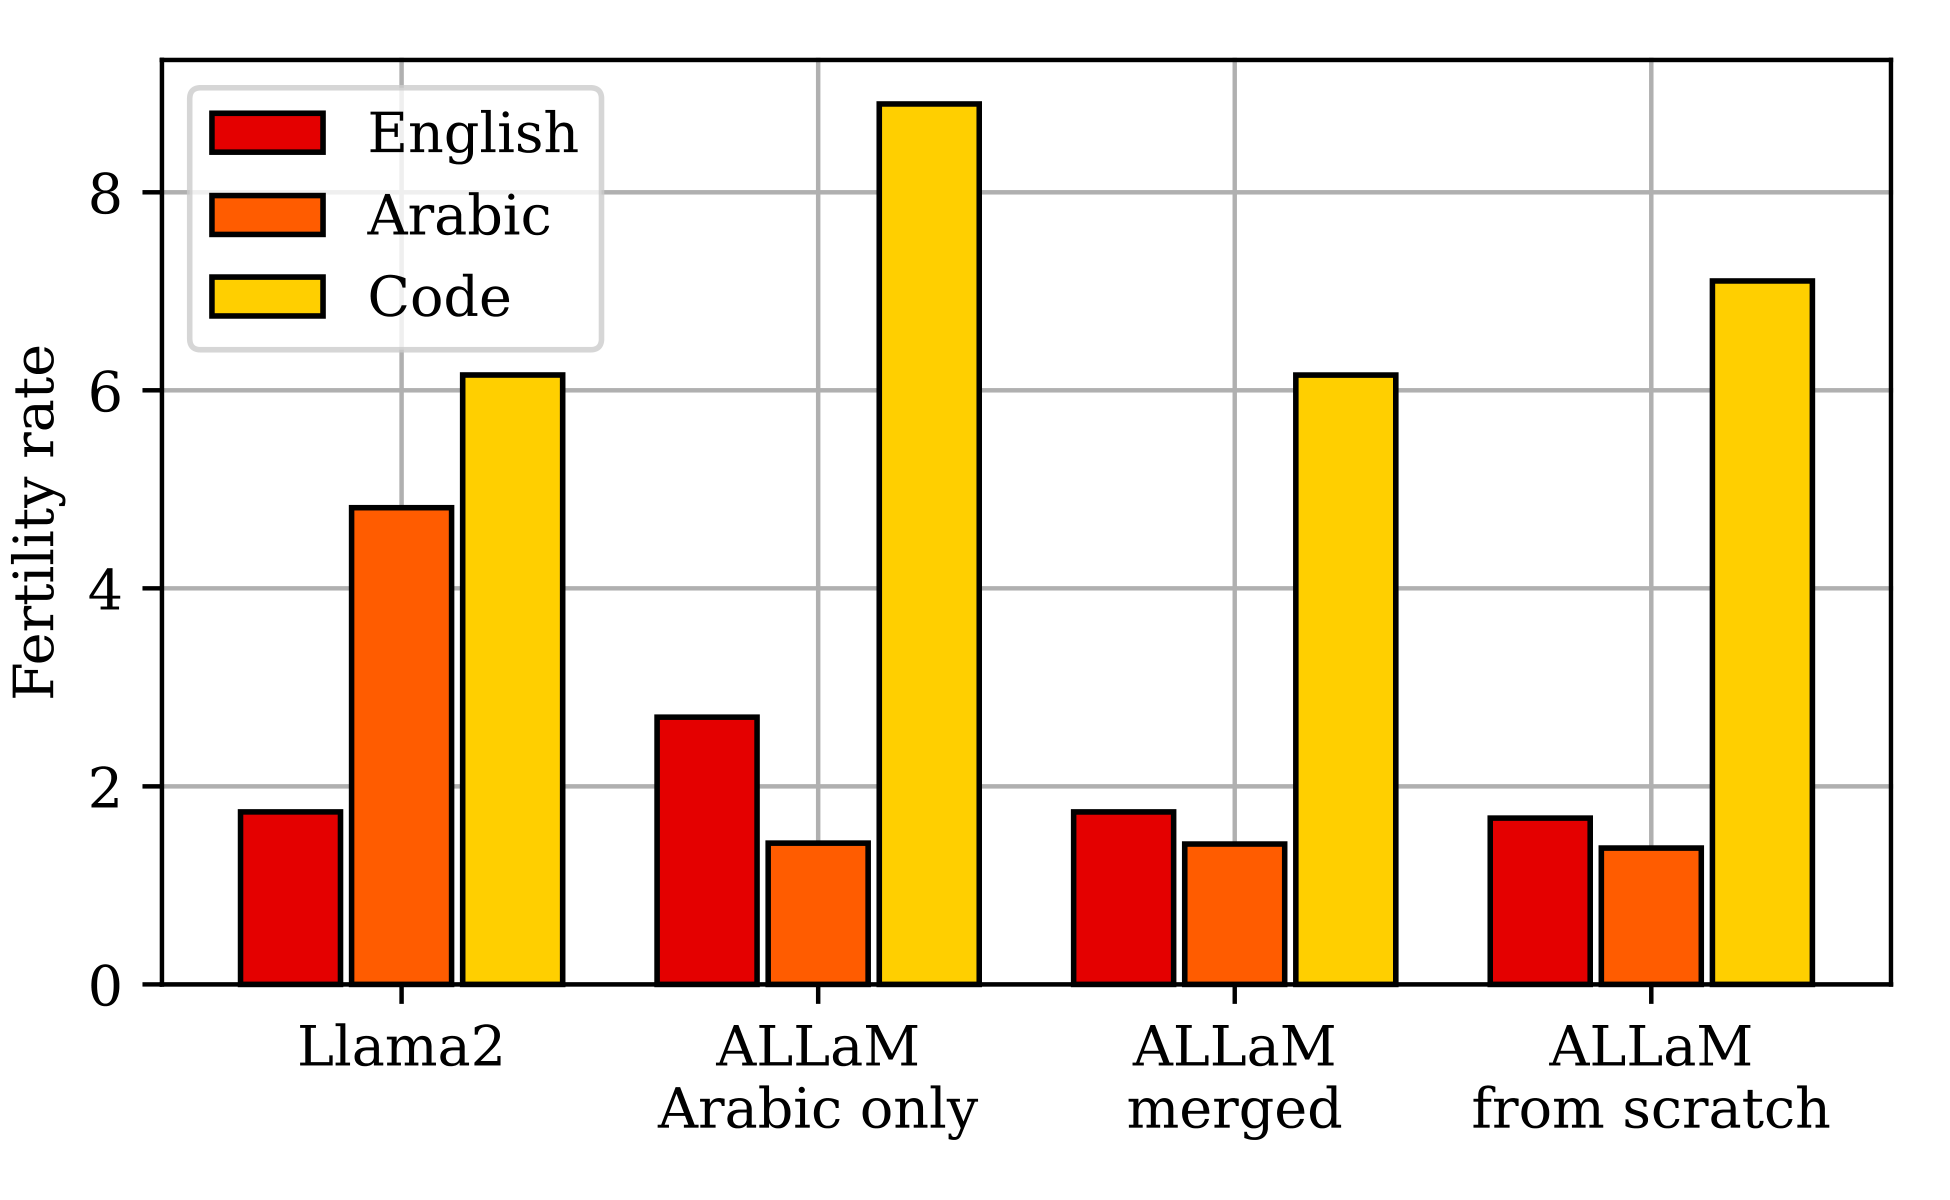
\includegraphics[width=\linewidth,height=0.48\textheight,keepaspectratio]{images/nlp-security-enterprise/allam_fig3_tokenizer_fertility.png}\\[0.2em]
      {\scriptsize Fertility of four tokenizers on English, Arabic and code. Bari et al., ``ALLaM: Large Language Models for Arabic and English,'' \href{https://arxiv.org/abs/2407.15390v1}{arXiv:2407.15390v1}, Figure~3.\par}
  \end{columns}
\end{frame}

\begin{frame}{Prompted Generalists Versus Specialist Models}
  \begin{columns}[T,onlytextwidth]
    \column{0.58\textwidth}
      \begin{itemize}\scriptsize\itemsep0.35em
        \item[\textcolor{red}{$\blacktriangleright$}] \textbf{Medprompt:} GPT-4 with no fine-tuning and three general prompting steps. Retrieve the 5 training questions nearest the test question as few-shot examples; give each a chain-of-thought rationale written by GPT-4, kept only if its answer matched the label; vote over 5 runs with the answer options shuffled (self-consistency, covered earlier).
        \item[\textcolor{red}{$\blacktriangleright$}] On MedQA (US medical licensing questions): 81.7\% zero-shot, 90.2\% with Medprompt, against 86.5\% for the fine-tuned Med-PaLM~2, ``a 27\% reduction in error rate''.
        \item[\textcolor{red}{$\blacktriangleright$}] \textbf{Finance:} GPT-4 beat BloombergGPT (covered earlier) on commodity-news headline classification, 86.0 against 82.2 weighted F1, yet a fine-tuned BERT scored 95.4. On entity recognition in financial agreements, a conditional random field (a classic sequence tagger) trained on in-domain text scored 82.7 F1; GPT-4 scored 56.7.
        \item[\textcolor{red}{$\blacktriangleright$}] \textbf{Specialise for a reason you can name:} data that cannot leave the network, cost or latency at volume, a language the general model handles poorly, or a narrow structured task. Re-run the comparison whenever a new general model ships.
      \end{itemize}
    \column{0.40\textwidth}
      \centering
      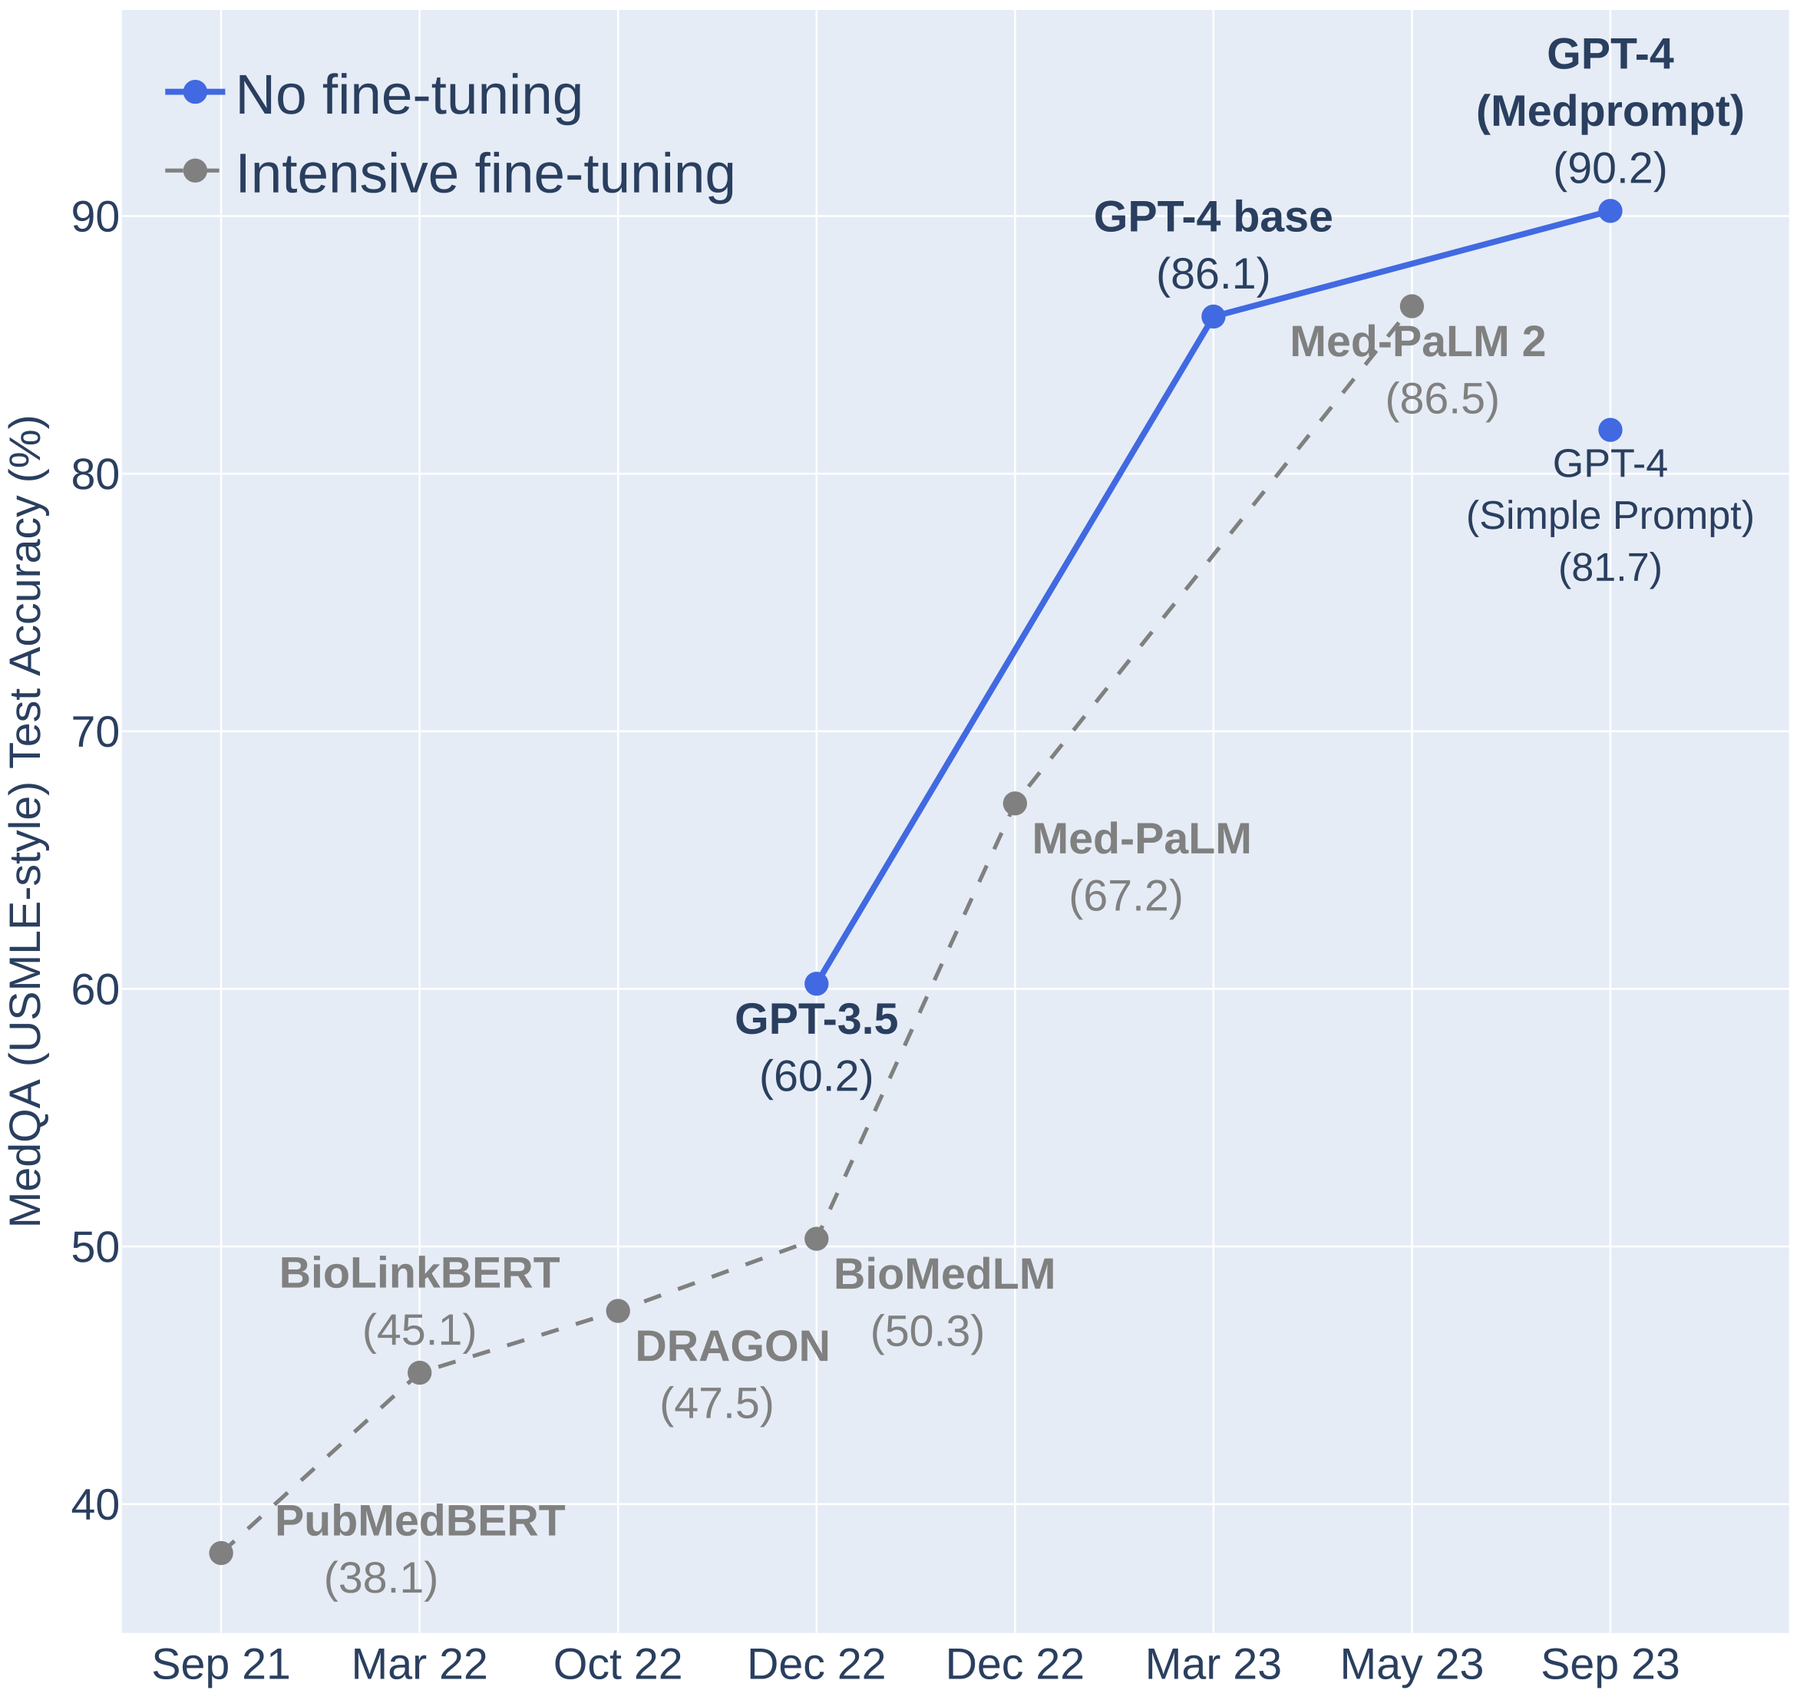
\includegraphics[width=\linewidth,height=0.55\textheight,keepaspectratio]{images/nlp-security-enterprise/medprompt_fig1a_medqa_specialists_vs_generalists.png}\\[0.2em]
      {\scriptsize MedQA accuracy over time: fine-tuned specialists (grey), general models (blue). Nori et al., ``Can Generalist Foundation Models Outcompete Special-Purpose Tuning? Case Study in Medicine,'' \href{https://arxiv.org/abs/2311.16452v1}{arXiv:2311.16452v1}, Figure~1(a).\par}
  \end{columns}
  \vspace{0.1em}
  {\scriptsize Li et al., ``Are ChatGPT and GPT-4 General-Purpose Solvers for Financial Text Analytics? A Study on Several Typical Tasks,'' EMNLP 2023 Industry Track, \href{https://arxiv.org/abs/2305.05862v2}{arXiv:2305.05862v2}, Tables~5 and~6.}
\end{frame}

\begin{frame}{RAFT: Fine-Tuning for Domain RAG}
  \begin{columns}[T,onlytextwidth]
    \column{0.55\textwidth}
      \begin{itemize}\scriptsize\itemsep0.3em
        \item[\textcolor{red}{$\blacktriangleright$}] \textbf{RAFT} (retrieval-augmented fine-tuning) trains on what the model sees at test time: a question plus retrieved documents. The \textbf{golden document} $D^{*}$ contains the answer; a \textbf{distractor document} $D_i$ does not:
          \[ \begin{aligned} P\%\text{ of examples:}&\quad Q + D^{*} + D_1 + \dots + D_k \rightarrow A^{*}\\ (1-P)\%\text{ of examples:}&\quad Q + D_1 + \dots + D_k \rightarrow A^{*} \end{aligned} \]
          $Q$ is the question, $k$ the number of distractors, and $A^{*}$ a chain-of-thought answer that quotes its evidence between \texttt{\#\#begin\_quote\#\#} and \texttt{\#\#end\_quote\#\#}.
        \item[\textcolor{red}{$\blacktriangleright$}] Leaving $D^{*}$ out of some examples can help: the best $P$ was 40\%, 60\% or 100\%, depending on the dataset. Training used four distractors per question.
        \item[\textcolor{red}{$\blacktriangleright$}] LLaMA2-7B with RAFT against the same model fine-tuned on domain questions without documents, then given RAG: 35.28 vs 4.41 on HotpotQA, 74.00 vs 42.59 on HuggingFace API calls. RAFT beat GPT-3.5 with RAG on four of five datasets, though not on HotpotQA (41.5). Without the chain of thought, HotpotQA fell 9.66 points.
      \end{itemize}
    \column{0.43\textwidth}
      \centering
      {\scriptsize
      \begin{tabular}{>{\raggedright\arraybackslash}p{3.0cm} >{\raggedright\arraybackslash}p{2.1cm}}
        \toprule
        \textbf{Signal in your evaluation} & \textbf{Rung to try} \\
        \midrule
        Facts change weekly; answers must cite a source & RAG \\
        \addlinespace[0.15em]
        Wrong format, tone or task behaviour & SFT or LoRA \\
        \addlinespace[0.15em]
        Unfamiliar terms; words split into many tokens & continued pretraining, vocabulary extension \\
        \addlinespace[0.15em]
        Right passage retrieved, answer misled by the others & RAFT \\
        \addlinespace[0.15em]
        Data may not leave the network & open weights on premises (on-premises section) \\
        \addlinespace[0.15em]
        A prompted general model already passes & stop; retest on each new model \\
        \bottomrule
      \end{tabular}\par}
  \end{columns}
  \vspace{0.1em}
  {\scriptsize Zhang et al., ``RAFT: Adapting Language Model to Domain Specific RAG,'' COLM 2024, \href{https://openreview.net/forum?id=rzQGHXNReU}{openreview.net}, Tables~1 and~2; preprint \href{https://arxiv.org/abs/2403.10131v2}{arXiv:2403.10131v2}.\par}
\end{frame}
